\documentclass[english,14pt]{beamer}
\usetheme{EastLansing}
\usecolortheme{spruce}

\usepackage{xcolor}
\usepackage{listings}
\usepackage{courier}
\usepackage{graphicx}
\usepackage{amsmath}
\usepackage{algorithm2e}
\usepackage{multicol}
\usepackage{hyperref}
\usepackage{textcomp}

% http://mirrors.ibiblio.org/CTAN/macros/latex/contrib/datetime2/datetime2.pdf
\usepackage{babel}
\usepackage[useregional]{datetime2}

% https://tex.stackexchange.com/questions/42619/x-mark-to-match-checkmark
\usepackage{pifont}% http://ctan.org/pkg/pifont

%% https://stackoverflow.com/questions/1435837/how-to-remove-footers-of-latex-beamer-templates
%%gets rid of bottom navigation bars
%\setbeamertemplate{footline}[page number]
%
%gets rid of navigation symbols
\setbeamertemplate{navigation symbols}{}


\usefonttheme[onlymath]{serif}

\definecolor{mGreen}{rgb}{0,0.6,0}
\definecolor{mGray}{rgb}{0.5,0.5,0.5}
\definecolor{mPurple}{rgb}{0.8,0,0.82}
\definecolor{backgroundColour}{rgb}{0.95,0.95,0.92}
\definecolor{lightBlue}{rgb}{0.1, 0.1, 0.8}

\newcommand\red[1]{{\color{red} #1}}
\newcommand\green[1]{{\color{green} #1}}
\newcommand\blue[1]{{\color{blue} #1}}

\newcommand{\cmark}{\ding{51}}%
\newcommand{\xmark}{\ding{55}}%

\lstdefinestyle{CStyle}{
    backgroundcolor=\color{backgroundColour},   
    commentstyle=\color{mGreen},
    keywordstyle=\color{magenta},
    numberstyle=\tiny\color{mGray},
    stringstyle=\color{mPurple},
    basicstyle=\footnotesize,
    breakatwhitespace=false,         
    breaklines=true,                 
    captionpos=b,                    
    keepspaces=true,                 
    numbers=left,                    
    numbersep=5pt,                  
    showspaces=false,                
    showstringspaces=false,
    showtabs=false,                  
    tabsize=2,
    language=Python
}

\lstdefinestyle{pseudo}{
        basicstyle=\ttfamily\footnotesize,
        keywordstyle=\color{lightBlue},
        morekeywords={BEGIN,END,IF,ELSE,ENDIF,ELSEIF,PRINT,WHILE,RETURN,ENDWHILE,DO,FOR,TO,IN,ENDFOR,BREAK,INPUT,CONDITIONS},
        morecomment=[l]{//},
        commentstyle=\color{mGreen}
}

\lstset{basicstyle=\footnotesize\ttfamily,breaklines=true}
\lstset{framextopmargin=50pt,tabsize=2}

\title{ENGG1003 - Thursday Week 8}
\subtitle{Numerical integration }%\\ \& computing integrals}
\author{Steve Weller}
\institute{University of Newcastle}
%\date{\today}
\date{29 April 2021}

% following is a bit of a hack, but forces page numbers (technically: frame numbers) to run 1,2,3,... 
% with titlepage counting as frame 1

\addtocounter{framenumber}{1}
\titlepage

\begin{document}

\begin{flushleft}
{\scriptsize Last compiled:~\DTMnow}
\vspace*{-5mm}
\end{flushleft}
\framebreak

%==============================================================

\begin{frame}[fragile]

\frametitle{Lecture overview}
\begin{enumerate}
	\item Basic ideas of numerical integration \red{\S6.1}
	\begin{itemize}
		\item engineering applications
		\item terminology
		\item additivity
	\end{itemize}
	
	\item[]
	
	\item Trapezoidal method \red{\S6.2}
	
	\item[]
	
	\item Midpoint method \red{\S6.3}
	
	\item[]
	
	\item Simpson's rule
	
\end{enumerate}

\end{frame}

%==============================================================

\begin{frame}[fragile]

\frametitle{$1)$ Basic ideas of numerical integration}

\begin{itemize}
	\item xxx
\end{itemize}

\end{frame}

%==============================================================

\begin{frame}[fragile]

\frametitle{$2)$ Trapezoidal method}

\begin{itemize}
	\item simple four-panel example on pp.~134--135
	\item Python code for simple example
	\item use \texttt{fill\_between} ??
% https://www.kite.com/python/docs/matplotlib.pyplot.fill_between
\end{itemize}

\begin{figure}[ht]
	\centering
	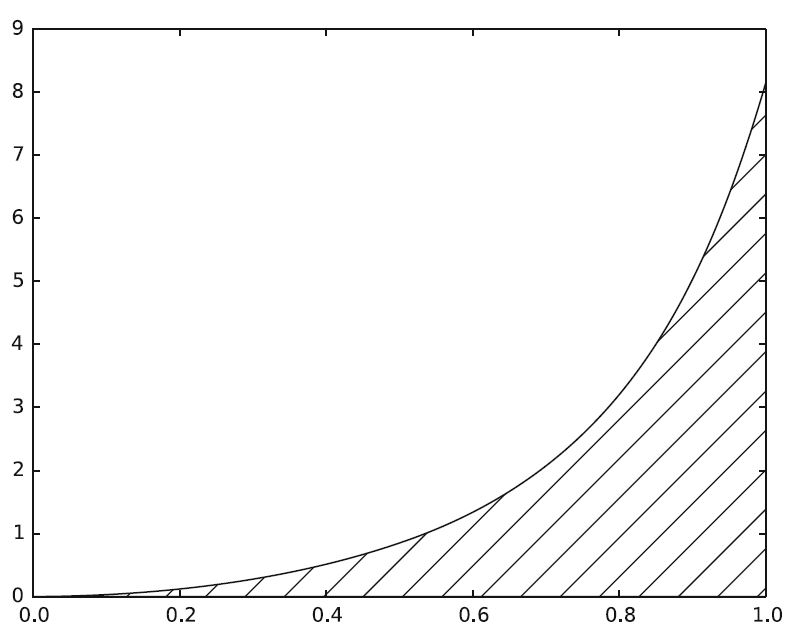
\includegraphics[width=0.5\textwidth]{figures/LLp134}
\end{figure}

\end{frame}

%%==============================================================
%
%\begin{frame}[fragile]
%
%\frametitle{}
%
%\begin{figure}[ht]
%	\centering
%	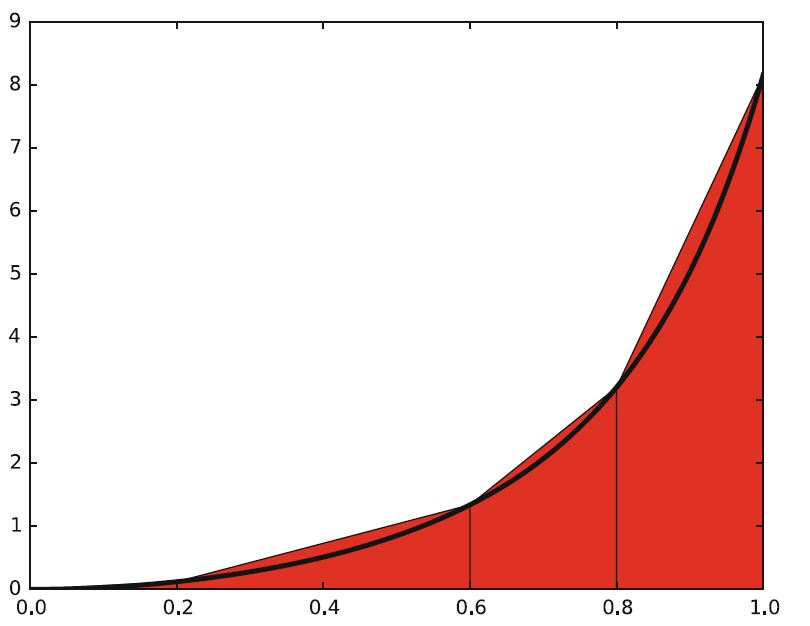
\includegraphics[width=0.5\textwidth]{figures/LLp135}
%\end{figure}
%
%\begin{itemize}
%	\item xxx
%\end{itemize}
%
%\end{frame}

%==============================================================

\begin{frame}[fragile]

\frametitle{}

\begin{figure}[ht]
	\centering
	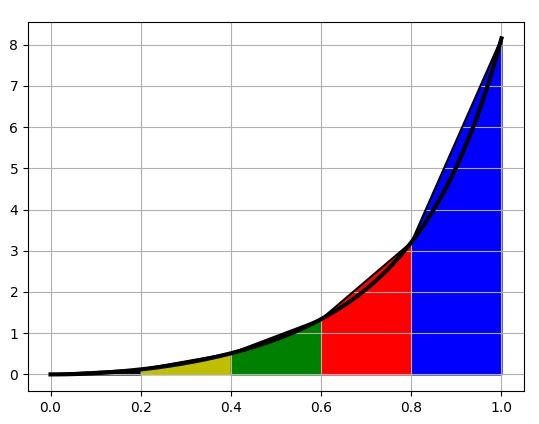
\includegraphics[width=0.7\textwidth]{figures/fivePanel}
\end{figure}

\begin{itemize}
	\item xxx
\end{itemize}

\end{frame}

%==============================================================

\begin{frame}[fragile]

\frametitle{$3)$ Midpoint method}

\begin{itemize}
	\item xxx
\end{itemize}

\end{frame}

%==============================================================

\begin{frame}[fragile]

\frametitle{$4)$ Simpson's rule}

\begin{itemize}
	\item xxx
\end{itemize}

\end{frame}

%==============================================================

\begin{frame}[fragile]

\frametitle{Lecture summary}

\begin{enumerate}
	\item Basic ideas of numerical integration
	
	\item[]
	
	\item Trapezoidal method \red{\S6.2}
	
	\item[]
	
	\item Midpoint method \red{\S6.3}
	
	\item[]
	
	\item Simpson's rule
	
\end{enumerate}

\end{frame}

%%==============================================================
%
%\begin{frame}[fragile]
%
%\frametitle{More information}
%\begin{itemize}
%	\item Newton's method in textbook \red{\S7.2}
%	\begin{itemize}
%		\item needs \emph{differentiation} from calculus (MATH1110)
%		\item in particular: need expression for \emph{tangent lines} to function $f(x)$, written as $f'(x)$
%	\end{itemize}
%
%	\item[]
%	
%	\item ``optimised'' versions of bisection and secant methods in textbook \red{\S7.3} and \red{\S7.4}
%	\begin{itemize}
%		\item maximise speed of computation by minimising number of function evaluations $f(x)$
%	\end{itemize}
%	
%	\item[]
%	
%	\item volume of truncated cone based on volumes of solids of revolution (needs calculus, MATH1110) \href{https://bit.ly/3sOsaj4}{https://bit.ly/3sOsaj4}
%\end{itemize}
%
%\end{frame}

\end{document}